\documentclass[tikz,border=20pt]{standalone}
\usepackage{amsmath, amssymb}

\begin{document}
	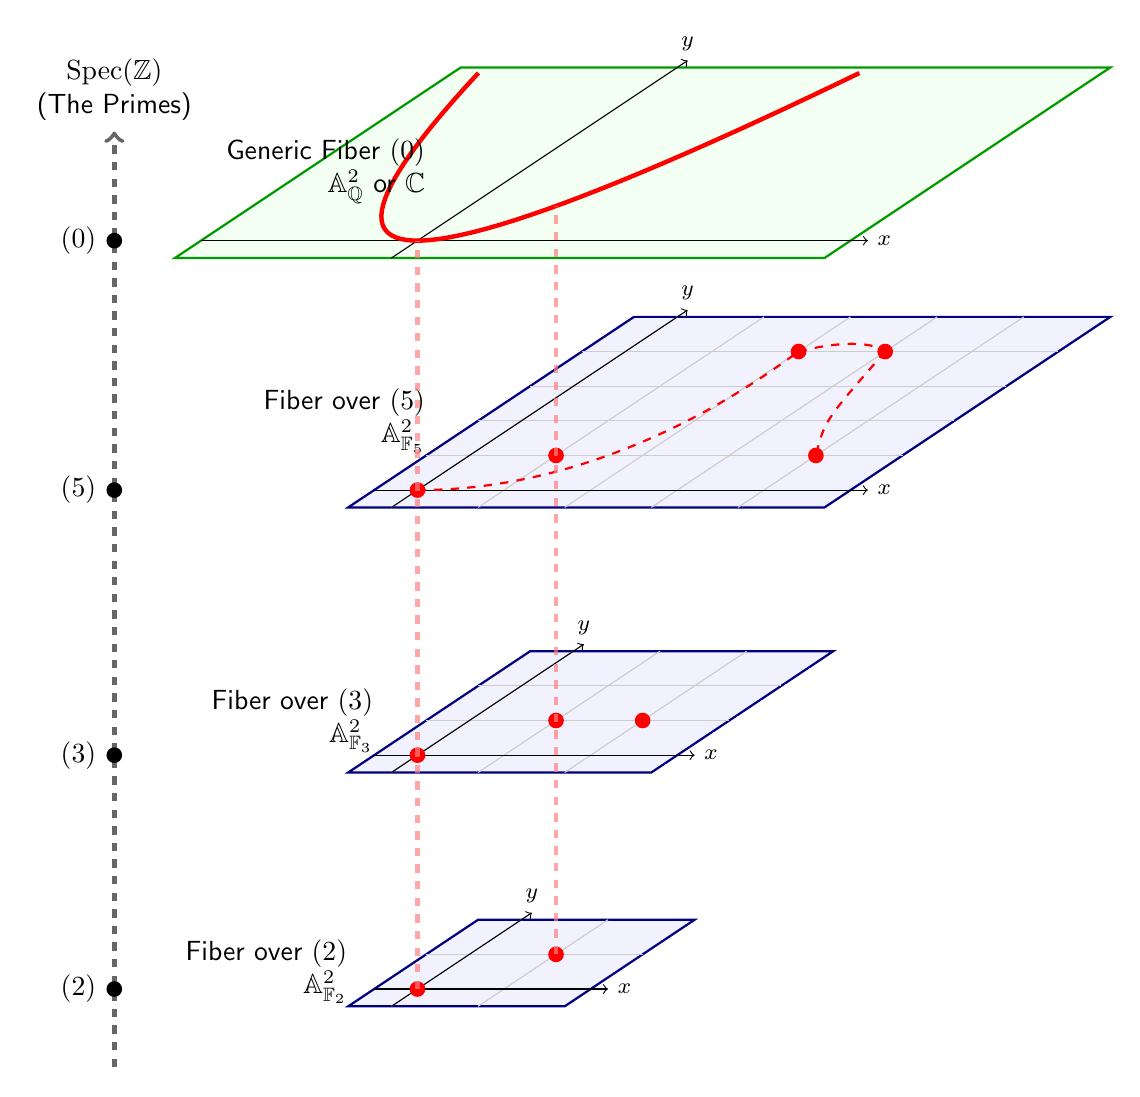
\begin{tikzpicture}[
		% Define our pseudo-3D axes: X is right, Y is up/right, Z is straight up
		x={(1cm, 0cm)}, 
		y={(0.6cm, 0.4cm)}, 
		z={(0cm, 1.8cm)},
		scale=1.1,
		font=\sffamily
		]
		
		% ==========================================
		% 1. The Global Base: Spec Z
		% ==========================================
		\draw[->, ultra thick, dashed, gray!80!black] (-3.5, 0, -0.5) -- (-3.5, 0, 5.5) 
		node[above, align=center, text=black] {$\operatorname{Spec}(\mathbb{Z})$\\(The Primes)};
		
		\node[circle, fill=black, inner sep=2pt, label=left:{$(2)$}] at (-3.5, 0, 0) {};
		\node[circle, fill=black, inner sep=2pt, label=left:{$(3)$}] at (-3.5, 0, 1.5) {};
		\node[circle, fill=black, inner sep=2pt, label=left:{$(5)$}] at (-3.5, 0, 3.2) {};
		\node[circle, fill=black, inner sep=2pt, label=left:{$(0)$}] at (-3.5, 0, 4.8) {};
		
		% ==========================================
		% 2. Fiber over p=2: The plane F_2[x,y]
		% ==========================================
		\begin{scope}[shift={(0,0,0)}]
			\draw[fill=blue!5, draw=blue!50!black, thick] (-0.5,-0.5) -- (2,-0.5) -- (2,2) -- (-0.5,2) -- cycle;
			
			% Grid
			\foreach \i in {0,1} {
				\draw[gray!40] (\i,-0.5) -- (\i,2);
				\draw[gray!40] (-0.5,\i) -- (2,\i);
			}
			% Axes
			\draw[->] (-0.5,0) -- (2.2,0) node[right, font=\footnotesize] {$x$};
			\draw[->] (0,-0.5) -- (0,2.2) node[above, font=\footnotesize] {$y$};
			
			% The graph y = x^2 mod 2 (Points: (0,0), (1,1))
			\node[circle, fill=red, inner sep=2pt] (p2_0) at (0,0) {};
			\node[circle, fill=red, inner sep=2pt] (p2_1) at (1,1) {};
			
			\node[left, align=right] at (-1, 0.5) {Fiber over $(2)$\\$\mathbb{A}^2_{\mathbb{F}_2}$};
		\end{scope}
		
		% ==========================================
		% 3. Fiber over p=3: The plane F_3[x,y]
		% ==========================================
		\begin{scope}[shift={(0,0,1.5)}]
			\draw[fill=blue!5, draw=blue!50!black, thick] (-0.5,-0.5) -- (3,-0.5) -- (3,3) -- (-0.5,3) -- cycle;
			
			% Grid
			\foreach \i in {0,1,2} {
				\draw[gray!40] (\i,-0.5) -- (\i,3);
				\draw[gray!40] (-0.5,\i) -- (3,\i);
			}
			% Axes
			\draw[->] (-0.5,0) -- (3.2,0) node[right, font=\footnotesize] {$x$};
			\draw[->] (0,-0.5) -- (0,3.2) node[above, font=\footnotesize] {$y$};
			
			% The graph y = x^2 mod 3 (Points: (0,0), (1,1), (2,1))
			\node[circle, fill=red, inner sep=2pt] (p3_0) at (0,0) {};
			\node[circle, fill=red, inner sep=2pt] (p3_1) at (1,1) {};
			\node[circle, fill=red, inner sep=2pt] (p3_2) at (2,1) {};
			
			\node[left, align=right] at (-1, 1) {Fiber over $(3)$\\$\mathbb{A}^2_{\mathbb{F}_3}$};
		\end{scope}
		
		% ==========================================
		% 4. Fiber over p=5: The plane F_5[x,y]
		% ==========================================
		\begin{scope}[shift={(0,0,3.2)}]
			\draw[fill=blue!5, draw=blue!50!black, thick] (-0.5,-0.5) -- (5,-0.5) -- (5,5) -- (-0.5,5) -- cycle;
			
			% Grid
			\foreach \i in {0,1,2,3,4} {
				\draw[gray!40] (\i,-0.5) -- (\i,5);
				\draw[gray!40] (-0.5,\i) -- (5,\i);
			}
			% Axes
			\draw[->] (-0.5,0) -- (5.2,0) node[right, font=\footnotesize] {$x$};
			\draw[->] (0,-0.5) -- (0,5.2) node[above, font=\footnotesize] {$y$};
			
			% The graph y = x^2 mod 5 (Points: (0,0), (1,1), (2,4), (3,4), (4,1))
			\node[circle, fill=red, inner sep=2pt] (p5_0) at (0,0) {};
			\node[circle, fill=red, inner sep=2pt] (p5_1) at (1,1) {};
			\node[circle, fill=red, inner sep=2pt] (p5_2) at (2,4) {};
			\node[circle, fill=red, inner sep=2pt] (p5_3) at (3,4) {};
			\node[circle, fill=red, inner sep=2pt] (p5_4) at (4,1) {};
			
			\node[left, align=right] at (-1, 2) {Fiber over $(5)$\\$\mathbb{A}^2_{\mathbb{F}_5}$};
			
			% Connecting the discrete dots visually to show the "ghost" parabola
			\draw[red, thick, dashed] (0,0) parabola (2,4);
			\draw[red, thick, dashed] (2,4) .. controls (2.5,4.5) and (3,4) .. (3,4);
			\draw[red, thick, dashed] (3,4) .. controls (3.5, 2) .. (4,1);
		\end{scope}
		
		% ==========================================
		% 5. The Generic Fiber: The plane Q[x,y] / C[x,y]
		% ==========================================
		\begin{scope}[shift={(0,0,4.8)}]
			\draw[fill=green!5, draw=green!60!black, thick] (-2.5,-0.5) -- (5,-0.5) -- (5,5) -- (-2.5,5) -- cycle;
			
			\draw[->] (-2.5,0) -- (5.2,0) node[right, font=\footnotesize] {$x$};
			\draw[->] (0,-0.5) -- (0,5.2) node[above, font=\footnotesize] {$y$};
			
			% The continuous graph y = x^2
			\draw[red, ultra thick, domain=-2.2:2.2, samples=50] plot (\x, {\x*\x});
			
			\node[left, align=right] at (-1, 2) {Generic Fiber $(0)$\\$\mathbb{A}^2_{\mathbb{Q}}$ or $\mathbb{C}$};
		\end{scope}
		
		% ==========================================
		% 6. The 3D Structure: Connecting the origin and (1,1) across fibers
		% ==========================================
		% The point (0,0) exists in every fiber
		\draw[red!50, ultra thick, dashed, opacity=0.7] 
		(0,0,0) -- (0,0,1.5) -- (0,0,3.2) -- (0,0,4.8);
		
		% The point (1,1) exists in every fiber
		\draw[red!50, ultra thick, dashed, opacity=0.7] 
		(1,1,0) -- (1,1,1.5) -- (1,1,3.2) -- (1,1,4.8);
		
	\end{tikzpicture}
\end{document}